\section*{Priority Quque~(continued)}

We finally give the pseudo-code for implementing the binary heap.
We not only maintain the array $S$ but also the number of elements in $S$, denoted as $n$.

\begin{minipage}{0.8\textwidth}
	\aaA {3}{function empty($PQ$)}\xxx
	\aab {if $n = 0$: return true;}\xxx
	\aab {else: return true;}\xxx
	\aaa {end function;}\xxx
\end{minipage}

\begin{minipage}{0.8\textwidth}
	\aaA {4}{function insert($PQ$, $x$)}\xxx
	\aab {$n = n + 1$;}\xxx
	\aab {$S[n] = x$;}\xxx
	\aab {bubble-up~($S$, $n$);}\xxx
	\aaa {end function;}\xxx
\end{minipage}

\begin{minipage}{0.8\textwidth}
	\aaA {2}{function find-min($PQ$)}\xxx
	\aab {return $S[1]$;}\xxx
	\aaa {end function;}\xxx
\end{minipage}

\begin{minipage}{0.8\textwidth}
	\aaA {4}{function delete-min($PQ$)}\xxx
	\aab {$S[1] = S[n]$;}\xxx
	\aab {$n = n - 1$;}\xxx
	\aab {sift-down~($S$, $1$);}\xxx
	\aaa {end function;}\xxx
\end{minipage}

\begin{minipage}{0.8\textwidth}
	\aaA {3}{function decrease-key($PQ$, $k$, new-key)}\xxx
	\aab {$S[k].key = $ new-key;}\xxx
	\aab {bubble-up~($S$, $k$);}\xxx
	\aaa {end function;}\xxx
\end{minipage}

Both bubble-up and sift-down procedures runs in $O(\log n)$ time.
This is because, a complete binary tree with $n$ vertices has a height of $\log n$, while
the worst case of either procedure traverses along a path between the root and a leaf.
Formally, in each recursive call, $k$ is either halved or doubled, and hence the number
of recursive calls is $\log n$.
The empty and find-min procedures takes $\Theta(1)$ time; the other 3 procedures takes $O(\log n)$ time, as they are dominated by either bubble-up or sift-down.

%\section*{Shortest Path Problems}
\section*{Single-Source Shortest Path Problem with Unit Edge Length}

In many applications, edges of graphs are associated with \emph{lengths}.
We will consider three cases.
\vspace*{-\topsep}
\begin{enumerate}
\item unit edge length: the length of each edge is 1;
\item positive edge length: the length of each edge is a positive number;
\item length of edge might be a negative number.
\end{enumerate}

Let $G = (V, E)$ be a graph; let $l(e)$ be the length of $e\in E$~(in any of above cases).
Let $p$ be a path of $G$. We define the length of path $p$, still denoted as $l(p)$,
as the sum of the length of all edges in $p$, i.e., $l(p) := \sum_{e\in p} l(e)$.
Given $u,v\in V$, the \emph{shortest path} from $u$ to $v$, is the path from $u$ to $v$
with smallest length. We use notation $distance(u,v)$ to denote the length
of the shortest path from $u$ to $v$.

%%%Shortest path admits the following \emph{optimal substructure} property.
%%%Intuitively, this property states that, the shortest path from $u$ to $v$
%%%contains the shortest path from $u$ to any internal vertex on this path~(formally described below).
%%%Essentially, this is why shortest path problem can be solved efficiently.
%%%
%%%\begin{property}
%%%Let $p = (v_1, v_2) \to (v_2, v_3) \to \cdots \to (v_{k-1}, v_k)$
%%%be the shortest path from $v_1$ to $v_k$.
%%%Then for any $1\le i \le k$,
%%%$p_i := (v_1, v_2) \to (v_2, v_3) \to \cdots \to (v_{i-1}, v_i)$, i.e., the portion of $p$ from $v_1$ to $v_i$,
%%%is the shortest path from $v_1$ to $v_i$.
%%%\end{property}
%%%
%%%\emph{Proof.} Suppose that 
%%%$p_i = (v_1, v_2) \to (v_2, v_3) \to \cdots \to (v_{i-1}, v_i)$
%%%is not the shortest path from $v_1$ to $v_i$. Assume that
%%%$q$ is the shorest path from $v_1$ to $v_i$.
%%%Then we can construct a path from $v_1$ to $v_k$ shorter than $p$,
%%%by concatenating $q$ and $(v_i, v_{i+1}) \to \cdots \to (v_{k-1}, v_k)$.
%%%This contradicts to the fact that $p$ is the shortest path from $v_1$ to $v_k$.\qed
%%%
%%%Note that the above property holds even for graphs with negative edge length~(as
%%%in the proof we don't assume anything about edge length).

There are different variants of shortest path problems.
One category is \emph{single-source shortest path problem}, where
we are given graph $G = (V, E)$ with edge length~(one of the three cases)
and a \emph{source} vertex $s\in V$, and we seek to find the shortest
path from $s$ to \emph{all} vertices.


We first solve the easiest version of shortest path problem: 
given $G = (V, E)$ with unit edge length and a \emph{source} vertex $s\in V$,
to find the shortest path from $s$ to all vertices, i.e., to find $distance(s, v)$ for any $v\in V$.

The breadth-first search~(BFS) can solve above problem. The idea of BFS
is to traverse the vertices of graph in increasing order of their distance from $s$.
Formally, we define $V_k$, $k = 0, 1, 2, \cdots$, as the subset of
vertices whose distance~(from $s$) is exactly $k$, i.e., $V_k = \{v \in V \mid distance(s, v) = k\}$.
BFS will first traverse vertices in $V_0$, then vertices in $V_1$, then $V_2$, and so on,
until all vertices reachable from $s$ are traversed.

Notice that $V_0 = \{s\}$ as $distance(s, s) = 0$.
How about $V_1$? They are the vertices reachable from $s$ with one edge~(but cannot be $s$), i.e., $V_1 = \{v \in V \mid (s, v) \in E\}\setminus V_0$.
How about $V_2$? They are the vertices reachable from some vertex in $V_1$ with one edge, but not in $V_0$ or $V_1$, i.e., $V_2 = \{v \in V \mid u\in V_1 \textrm{ and } (u, v) \in E\} \setminus (V_0\cup V_1)$.
The general form is that $V_{k + 1} = \{v \in V \mid u \in V_k \textrm{ and } (u, v) \in E\} \setminus (V_0\cup V_1 \cup \cdots \cup V_k)$.
This suggests an iterative framework of BFS: to find $V_{k+1}$, explore the out-edges of $V_k$ to collect the \emph{newly} reached 
vertices~(i.e., those not in $V_0\cup V_1 \cup \cdots \cup V_k$).
To realize this idea, BFS uses two data structures; the complete algorithm follows. 
\vspace*{-\topsep}
\begin{enumerate}
\item Array $dist$ of size $|V|$, initialized as $dist[v] = \infty$ for any $v\in V$.
Array $dist$ serves as two purposes: indicating a vertex has been reached or not,
and storing the distance from $s$~(after it has been reached).
Formally, before $v$ is reached, $dist[v] = \infty$;
after $v$ is reached, $dist[v] = distance~(s, v)$.

\item Queue $Q$, which stores the vertices haven't been explored.
Vertices will be added to $Q$ in the order of $V_0, V_1, V_2, \cdots$,
and vertices will be deleted from $Q$ in the same order~(as queue is first-in-first-out).
%At the time $v$ is deleted from $Q$, BFS explores it: examine out-edges of $v$,
%set $dist$ value for newly reached vertices, and add them to $Q$.
\end{enumerate}

%The complete BFS algorithm is given below.

\begin{minipage}{0.8\textwidth}
	\aaA {15}{Algorithm BFS~($G = (V, E), s \in V$)}\xxx
	\aab {$dist[v] = \infty$, for any $v\in V$;}\xxx
	\aab {init an empty queue $Q$;}\xxx
	\aab {$dist[s] = 0$;}\xxx
	\aab {insert~($Q, s$);}\xxx
	\aaB {9}{while~(empty~($Q$) = false)}\xxx
	\aac {$u$ = find-earliest~($Q$);}\xxx
	\aac {delete-earliest~($Q$);}\xxx
	\aaC {5}{for each edge~$(u, v)\in E$}\xxx
	\aaD {3}{if~($dist[v] = \infty$)}\xxx
	\aae {$dist[v] = dist[u] + 1$;}\xxx
	\aae {insert~($Q$, $v$);}\xxx
	\aad {end if;}\xxx
	\aac {end for;}\xxx
	\aab {end while;}\xxx
	\aaa {end algorithm;}\xxx
\end{minipage}




Initially BFS has $V_0$~(i.e., $s$) in $Q$~(right before the while loop), 
then BFS deletes $s$ from $Q$ and explores $s$~(newly reached vertices---these are $V_1$, will have their $dist$ set as 1 and be added to $Q$);
at the time of finishing exploring $V_0$, $V_1$ will be in $Q$. 
Next, BFS will gradually delete and explore each of the vertices in $Q$~(i.e., $V_1$);
in this process, vertices in $V_2$ will be reached, their $dist$ be set as 2, and be added to $Q$;
after all of them are deleted and explored, $Q$ will exactly consist of $V_2$.

In general, BFS keeps the following invariant: for every $k = 0, 1, 2, \cdots$, 
there is a time at which $Q$ contains exactly $V_k$, $dist[v] = distance(s, v)$ for any $v\in V_0\cup V_1\cup \cdots V_k$,
and $dist[v] = \infty$ for all other vertices.
This invariant explains the behavior of BFS while also proves its correctness:
when the $Q$ becomes empty, $dist[v] = distance(s, v)$ for any $v\in V$.

Following above invariant and the pseudo-code, we know that the time that vertex $v$ is reached for the first time~(happend when $(u,v)\in E$ is checked and $dist[v] = \infty$),
is also the time that the shortest path to $v$ is found, that the $dist[v]$ gets assigned, and that $v$ is added to $Q$.


BFS runs in $O(|V| + |E|)$ time, as each vertex will be explored at most once, and each 
edge will be examined at most once~(for directed graph) and at most twice~(for undirected graph).
Note that BFS~($G$, $s$) only traverses those vertices in $G$ can be reached from $s$.


\section*{Single-Source Shortest Path Problem with Positive Edge Length}

We now study the single-source shortest path problem with positive edge length:
given graph $G = (V, E)$ with edge length $l(e) > 0$ for any $e\in E$ and
source vertex $s\in V$, to seek $distance(s, v)$ for any $v\in V$.
We solve this problem with the \emph{Dijkstra's algorithm}.

Similar to BFS, the idea of Dijkstra's algorithm is also to
determine and calculate the distance of each vertex
in increasing order of distance.
More specifically, let $(v_1^*, v_2^*, \cdots, v_n^*)$, $n = |V|$,
be the order of vertices with increasing distance, i.e., $distance(s, v_k^*) \le distance(s, v_{k+1}^*)$, $1\le k < n$.
In other words, we define $v_k^*$ as the $k$-th closest vertex from $s$.
We don't know this order in advance.
But Dijktra's algorithm will identify vertices in this order and calculate
their distance.
For the sake of writing and notations, we define $R_k = \{v_1^*, v_2^*, \cdots, v_k^*\}$, i.e., 
the first $k$ vertices in above list; $R_k$ are also the closest $k$ vertices from $s$.

Clearly, $v_1^* = s$, $distance(s, v_1^*) = distance(s, s) = 0$, and $R_1 = \{s\}$.
The key question is: given $R_k$~(i.e., the closest $k$ vertices from $s$) and their distances~(i.e., $distance(s, v)$ for every $v\in R_k$),
how to find $v_{k + 1}^*$?
Below we show that $v_{k + 1}^*$ must be within \emph{one-edge extension} of $R_k$.
\begin{claim}
There must exist vertex $u\in R_k$ such that $(u, v_{k+1}^*) \in E$.
\end{claim}
\emph{Proof.} Suppose conversely that for every $u\in R_k$ we have $(u, v_{k+1}^k)\not\in E$.
Consider the shortest path from $s$ to $v_{k+1}^*$.
Let $w$ be the vertex right before $v_{k+1}^*$ in path $p$, i.e, $(w, v_{k+1}^*)$ is the last edge of $p$.
We have $distance(s, v_{k+1}^*) = distance(s, w) + l(w, v_{k+1}^*)$. %following the optimal substructure property.
As edges have positive edge length, we have $l(w, v_{k+1}^*) > 0$, and consequently
$distance(s, w) < distance(s, v_{k+1}^*)$.
Besides, according to the assumption, we have $w\not\in R_k$.
Therefore, $v_{k+1}^*$ cannot be the $(k+1)$-th closest vertex from $s$,
because $w$ has a shorter distance than $v_{k+1}^*$. This contradicts to the definition of $v_{k+1}^*$.\qed

Note that, in above proof, we use the fact that edges have positive lengths.
Hence, above claim may not be true for graphs with negative edge length.
This also explains why Dijkstra's algorithm won't work for graphs with negative edge length.


The above claim shows that, the last edge $(u,v)$ of the shortest path from $s$ to $v_{k+1}^*$
satisfies that $u\in R_k$ and $v\not\in R_k$. Which such edge is the correct one?
We don't know, so we enumerate all such edges $(u,v)\in E$ with $u\in R_k$ and $v\not\in R_k$.
Suppose that $(u,v)$ is the last edge of the shortest path from $s$ to $v_{k+1}^*$,
%then following the optimal substructure property,
we know that $distance(s,v) = distance(s,u) + l(u,v)$.
This leads to the following formula to calculate $v_{k+1}^*$ and its predecessor in the shortest path.
See an example in Figure~\ref{fig:extension}.


\begin{corollary} \label{cor1}
We have 
$$distance(s, v_{k+1}^*) = \textstyle \min_{u\in R_k, v\in V \setminus R_k, (u, v)\in E} (distance(s, u) + l(u,v)).$$
Let $(u',v')$ be the optimal edge in the minimization, i.e.,
$$(u',v') := \textstyle \arg\min_{u\in R_k, v\in V \setminus R_k, (u, v)\in E} (distance(s, u) + l(u,v)).$$
Then $v_{k+1}^* = v'$ and $u'$ is the predecessor of $v_{k+1}^*$ in the shortest path from $s$ to $v_{k+1}^*$.
\end{corollary}


\begin{figure}[h]
\centering{

\tikzset{every picture/.style={line width=0.75pt}} %set default line width to 0.75pt        

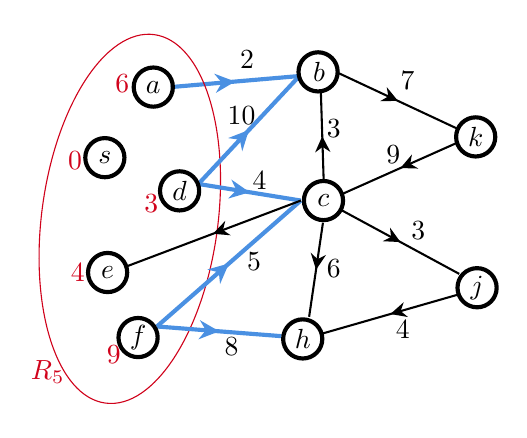
\begin{tikzpicture}[x=0.5pt,y=0.5pt,yscale=-1,xscale=1]
%uncomment if require: \path (0,296); %set diagram left start at 0, and has height of 296

%Straight Lines [id:da3320252336737717] 
\draw [color={rgb, 255:red, 74; green, 144; blue, 226 }  ,draw opacity=1 ][line width=1.5]    (119,48) -- (212,40) ;
\draw [shift={(165.5,44)}, rotate = 535.0799999999999] [fill={rgb, 255:red, 74; green, 144; blue, 226 }  ,fill opacity=1 ][line width=0.08]  [draw opacity=0] (14.56,-6.99) -- (0,0) -- (14.56,6.99) -- (9.67,0) -- cycle    ;
%Shape: Ellipse [id:dp2857420369455096] 
\draw  [color={rgb, 255:red, 208; green, 2; blue, 27 }  ,draw opacity=1 ] (26.24,134.88) .. controls (35.95,61.34) and (72.1,5.46) .. (106.98,10.07) .. controls (141.87,14.67) and (162.28,78.02) .. (152.57,151.56) .. controls (142.86,225.1) and (106.71,280.98) .. (71.83,276.37) .. controls (36.94,271.77) and (16.53,208.42) .. (26.24,134.88) -- cycle ;
%Straight Lines [id:da02943457575339692] 
\draw [color={rgb, 255:red, 74; green, 144; blue, 226 }  ,draw opacity=1 ][line width=1.5]    (139,118) -- (212,40) ;
\draw [shift={(175.5,79)}, rotate = 493.1] [fill={rgb, 255:red, 74; green, 144; blue, 226 }  ,fill opacity=1 ][line width=0.08]  [draw opacity=0] (14.56,-6.99) -- (0,0) -- (14.56,6.99) -- (9.67,0) -- cycle    ;
%Straight Lines [id:da7032022658079198] 
\draw [color={rgb, 255:red, 74; green, 144; blue, 226 }  ,draw opacity=1 ][line width=1.5]    (139,118) -- (213,130) ;
\draw [shift={(176,124)}, rotate = 189.21] [fill={rgb, 255:red, 74; green, 144; blue, 226 }  ,fill opacity=1 ][line width=0.08]  [draw opacity=0] (14.56,-6.99) -- (0,0) -- (14.56,6.99) -- (9.67,0) -- cycle    ;
%Straight Lines [id:da9416797747261806] 
\draw [color={rgb, 255:red, 74; green, 144; blue, 226 }  ,draw opacity=1 ][line width=1.5]    (109,221) -- (213,130) ;
\draw [shift={(161,175.5)}, rotate = 498.81] [fill={rgb, 255:red, 74; green, 144; blue, 226 }  ,fill opacity=1 ][line width=0.08]  [draw opacity=0] (14.56,-6.99) -- (0,0) -- (14.56,6.99) -- (9.67,0) -- cycle    ;
%Straight Lines [id:da6197316893700862] 
\draw [color={rgb, 255:red, 74; green, 144; blue, 226 }  ,draw opacity=1 ][line width=1.5]    (109,221) -- (199,228) ;
\draw [shift={(154,224.5)}, rotate = 184.45] [fill={rgb, 255:red, 74; green, 144; blue, 226 }  ,fill opacity=1 ][line width=0.08]  [draw opacity=0] (14.56,-6.99) -- (0,0) -- (14.56,6.99) -- (9.67,0) -- cycle    ;
%Straight Lines [id:da7705917014251779] 
\draw [color={rgb, 255:red, 0; green, 0; blue, 0 }  ,draw opacity=1 ][line width=0.75]    (86,178) -- (213,130) ;
\draw [shift={(149.5,154)}, rotate = 339.3] [fill={rgb, 255:red, 0; green, 0; blue, 0 }  ,fill opacity=1 ][line width=0.08]  [draw opacity=0] (11.61,-5.58) -- (0,0) -- (11.61,5.58) -- (7.71,0) -- cycle    ;
%Straight Lines [id:da7178806242260687] 
\draw [color={rgb, 255:red, 0; green, 0; blue, 0 }  ,draw opacity=1 ][line width=0.75]    (326,78) -- (240.5,38) ;
\draw [shift={(283.25,58)}, rotate = 205.07] [fill={rgb, 255:red, 0; green, 0; blue, 0 }  ,fill opacity=1 ][line width=0.08]  [draw opacity=0] (11.61,-5.58) -- (0,0) -- (11.61,5.58) -- (7.71,0) -- cycle    ;
%Straight Lines [id:da2873203830948724] 
\draw [color={rgb, 255:red, 0; green, 0; blue, 0 }  ,draw opacity=1 ][line width=0.75]    (326.5,88) -- (243.5,125) ;
\draw [shift={(285,106.5)}, rotate = 335.97] [fill={rgb, 255:red, 0; green, 0; blue, 0 }  ,fill opacity=1 ][line width=0.08]  [draw opacity=0] (11.61,-5.58) -- (0,0) -- (11.61,5.58) -- (7.71,0) -- cycle    ;
%Straight Lines [id:da9325647569597147] 
\draw [color={rgb, 255:red, 0; green, 0; blue, 0 }  ,draw opacity=1 ][line width=0.75]    (327.5,183) -- (242.5,137) ;
\draw [shift={(285,160)}, rotate = 208.42] [fill={rgb, 255:red, 0; green, 0; blue, 0 }  ,fill opacity=1 ][line width=0.08]  [draw opacity=0] (11.61,-5.58) -- (0,0) -- (11.61,5.58) -- (7.71,0) -- cycle    ;
%Straight Lines [id:da8240281406202591] 
\draw [color={rgb, 255:red, 0; green, 0; blue, 0 }  ,draw opacity=1 ][line width=0.75]    (219,214) -- (229,146) ;
\draw [shift={(224,180)}, rotate = 278.37] [fill={rgb, 255:red, 0; green, 0; blue, 0 }  ,fill opacity=1 ][line width=0.08]  [draw opacity=0] (11.61,-5.58) -- (0,0) -- (11.61,5.58) -- (7.71,0) -- cycle    ;
%Straight Lines [id:da6386544223700206] 
\draw [color={rgb, 255:red, 0; green, 0; blue, 0 }  ,draw opacity=1 ][line width=0.75]    (229,226) -- (326.5,198) ;
\draw [shift={(277.75,212)}, rotate = 343.98] [fill={rgb, 255:red, 0; green, 0; blue, 0 }  ,fill opacity=1 ][line width=0.08]  [draw opacity=0] (11.61,-5.58) -- (0,0) -- (11.61,5.58) -- (7.71,0) -- cycle    ;
%Straight Lines [id:da7268529078901531] 
\draw [color={rgb, 255:red, 0; green, 0; blue, 0 }  ,draw opacity=1 ][line width=0.75]    (229.5,115) -- (227.5,52) ;
\draw [shift={(228.5,83.5)}, rotate = 448.18] [fill={rgb, 255:red, 0; green, 0; blue, 0 }  ,fill opacity=1 ][line width=0.08]  [draw opacity=0] (11.61,-5.58) -- (0,0) -- (11.61,5.58) -- (7.71,0) -- cycle    ;

% Text Node
\draw (16,244) node [anchor=north west][inner sep=0.75pt]   [align=left] {$\displaystyle \textcolor[rgb]{0.82,0.01,0.11}{R}\textcolor[rgb]{0.82,0.01,0.11}{_{5}}$};
% Text Node
\draw (43,93) node [anchor=north west][inner sep=0.75pt]   [align=left] {$\displaystyle \textcolor[rgb]{0.82,0.01,0.11}{0}$};
% Text Node
\draw (167.24,20.06) node [anchor=north west][inner sep=0.75pt]   [align=left] {$\displaystyle 2$};
% Text Node
\draw  [line width=1.5]   (71.38, 99) circle [x radius= 14.15, y radius= 14.15]   ;
\draw (71.38,99) node   [align=left] {$\displaystyle s$};
% Text Node
\draw (77,37) node [anchor=north west][inner sep=0.75pt]   [align=left] {$\displaystyle \textcolor[rgb]{0.82,0.01,0.11}{6}$};
% Text Node
\draw  [line width=1.5]   (106.38, 48) circle [x radius= 14.15, y radius= 14.15]   ;
\draw (106.38,48) node   [align=left] {$\displaystyle a$};
% Text Node
\draw (98,124) node [anchor=north west][inner sep=0.75pt]   [align=left] {$\displaystyle \textcolor[rgb]{0.82,0.01,0.11}{3}$};
% Text Node
\draw  [line width=1.5]   (125.38, 123) circle [x radius= 14.15, y radius= 14.15]   ;
\draw (125.38,123) node   [align=left] {$\displaystyle d$};
% Text Node
\draw (45,174) node [anchor=north west][inner sep=0.75pt]   [align=left] {$\displaystyle \textcolor[rgb]{0.82,0.01,0.11}{4}$};
% Text Node
\draw  [line width=1.5]   (73.38, 182) circle [x radius= 14.15, y radius= 14.15]   ;
\draw (73.38,182) node   [align=left] {$\displaystyle e$};
% Text Node
\draw  [line width=1.5]   (225.48, 37) circle [x radius= 14.15, y radius= 14.15]   ;
\draw (219.98,37) node [anchor=west] [inner sep=0.75pt]   [align=left] {$\displaystyle b$};
% Text Node
\draw  [line width=1.5]   (229.38, 130) circle [x radius= 14.15, y radius= 14.15]   ;
\draw (229.38,130) node   [align=left] {$\displaystyle c$};
% Text Node
\draw  [line width=1.5]   (339.38, 84) circle [x radius= 14.15, y radius= 14.15]   ;
\draw (339.38,84) node   [align=left] {$\displaystyle k$};
% Text Node
\draw  [line width=1.5]   (214.38, 230) circle [x radius= 14.15, y radius= 14.15]   ;
\draw (214.38,230) node   [align=left] {$\displaystyle h$};
% Text Node
\draw (71,233) node [anchor=north west][inner sep=0.75pt]   [align=left] {$\displaystyle \textcolor[rgb]{0.82,0.01,0.11}{9}$};
% Text Node
\draw  [line width=1.5]   (95.38, 229) circle [x radius= 14.15, y radius= 14.15]   ;
\draw (95.38,229) node   [align=left] {$\displaystyle f$};
% Text Node
\draw  [line width=1.5]   (340.38, 193) circle [x radius= 14.15, y radius= 14.15]   ;
\draw (340.38,193) node   [align=left] {$\displaystyle j$};
% Text Node
\draw (158.24,60.06) node [anchor=north west][inner sep=0.75pt]   [align=left] {$\displaystyle 10$};
% Text Node
\draw (176.24,107.06) node [anchor=north west][inner sep=0.75pt]   [align=left] {$\displaystyle 4$};
% Text Node
\draw (172.24,166.06) node [anchor=north west][inner sep=0.75pt]   [align=left] {$\displaystyle 5$};
% Text Node
\draw (156,227.5) node [anchor=north west][inner sep=0.75pt]   [align=left] {$\displaystyle 8$};
% Text Node
\draw (283.24,35.06) node [anchor=north west][inner sep=0.75pt]   [align=left] {$\displaystyle 7$};
% Text Node
\draw (291,143) node [anchor=north west][inner sep=0.75pt]   [align=left] {$\displaystyle 3$};
% Text Node
\draw (279.75,215) node [anchor=north west][inner sep=0.75pt]   [align=left] {$\displaystyle 4$};
% Text Node
\draw (273,88.47) node [anchor=north west][inner sep=0.75pt]   [align=left] {$\displaystyle 9$};
% Text Node
\draw (230,70) node [anchor=north west][inner sep=0.75pt]   [align=left] {$\displaystyle 3$};
% Text Node
\draw (230,171) node [anchor=north west][inner sep=0.75pt]   [align=left] {$\displaystyle 6$};


\end{tikzpicture}

}
\caption{Example for Colollary~1. Suppose that we know $R_5 = \{s, a, d, e, f\}$ and their distances from $s$, marked next to vertices.
To find $v_6^*$ and calculate $distance(s,v_6^*)$, we consider all one-edge extension of $R_5$, marked as thick blue edges.
Following Corollary~1, $distance(s, v_6^*) = \min_{u\in R_5, v\not\in R_5, (u,v)\in E} (distance(s,u) + l(u,v)) = \min\{6 + 2, 3 + 10, 3 + 4, 9 + 5, 9 + 8\} = 7$,
and the optimal edge is $(d,c)$. Hence, $v_6^* = c$ and $d$ is the predecessor of $d$ in the shortest path.  }
\label{fig:extension}
\end{figure}


%Above Corollary offers a framework of Dijkstra's algorithm by sequentially calculating $v_k^*$ and $distance~(s, v_k^*)$ for $k = 1, 2, \cdots, n$.
%We will show details in realizing this framework by using efficient data structures.
We therefore have the following algorithm~(framework), in which we follow above formula
to iteratively construct $R_k$, $k = 1, 2, \cdots, n$.
We again use array $dist$ of size $n$ to store the distance for vertices in $R_k$.

\begin{minipage}{0.8\textwidth}
	\aaA {8}{Algorithm Dijkstra-Framework~($G = (V, E), s \in V$)}\xxx
	\aab {let $R_1 = \{s\}$;}\xxx
	\aab {$dist[s] = 0$; $dist[v] = \infty$ for any $v \neq s$;}\xxx
	\aaB {4}{for $k = 1 \to n-1$}\xxx
	\aac {calculate $(u',v') := \arg\min_{u\in R_k, v\in V \setminus R_k, (u, v)\in E} (dist[u] + l(u,v))$;}\xxx
	\aac {$R_{k+1} = R_k\cup \{v'\}$;}\xxx
	\aac {$dist[v'] = dist[u'] + l(u',v')$;}\xxx
	\aab {end for;}\xxx
	\aaa {end algorithm;}\xxx
\end{minipage}

A naive implementation of above framework takes $O(|V|\cdot|E|)$ time,
as for each $k$, the calculation of the minimization may take $O(|E|)$ time.
Next lecture, we will show how to use efficient data structures to speed up,
leading to the complete Dijkstra's algorithm with improved running time.
